\documentclass[conference]{IEEEtran}
\IEEEoverridecommandlockouts
% The preceding line is only needed to identify funding in the first footnote. If that is unneeded, please comment it out.
\usepackage{cite}
\usepackage{amsmath,amssymb,amsfonts}
\usepackage{algorithmic}
\usepackage{graphicx}
\usepackage{textcomp}
\usepackage{xcolor}
\usepackage{dblfloatfix}
\usepackage{flushend}
\usepackage{subcaption} %  for subfigures environments 
%\def\BibTeX{{\rm B\kern-.05em{\sc i\kern-.025em b}\kern-.08em
%    T\kern-.1667em\lower.7ex\hbox{E}\kern-.125emX}}
%\usepackage[all]{background}
%\usepackage{stackengine}
%\setstackEOL{\\}
%\setstackgap{L}{\normalbaselineskip}
%\SetBgContents{\color{blue}{\tiny \Longstack{PREPRINT - Accepted at the 43rd AIAA/IEEE Digital %Avionics Systems Conference (DASC), 2024.}}}% Set contents
%\SetBgPosition{4.5cm,1cm}% Select location
%\SetBgOpacity{1.0}% Select opacity
%\SetBgAngle{0}% Select rotation of logo
%\SetBgScale{1.8}% Select scale factor of logo

\begin{document}

\title{Evaluation of New Assurance Tools for Airborne Machine Learning-Based Functions\\
\thanks{Distribution statement ``A'' (approved for public release, distribution unlimited). This research was developed with funding from the Defense Advanced Research Projects Agency (DARPA), contract FA8750-18-C-0099. The views, opinions, or findings expressed are those of the authors and should not be interpreted as representing the official views or policies of the Department of Defense or the U.S. Government.}
}

\author{\IEEEauthorblockN{Cong Liu, Heber Herencia-Zapana, Saqib Hasan, Amer Tahat, Isaac Amundson,
        Darren Cofer}
\IEEEauthorblockA{\textit{Collins Aerospace} \\
\{first.last\}@collins.com}
}

\maketitle

\begin{abstract}
As part of the DARPA Assured Autonomy program, our team has developed or evaluated a number of technologies to address gaps in traditional hardware and software assurance processes that make it difficult or impossible to demonstrate the correctness and safety of machine learning (ML) components.    These include new approaches for testing and completeness metrics, formal analysis of neural networks, input domain shift assessment, and run-time monitoring and enforcement architectures.  Although many of these tools and methods were successfully applied to demonstration platforms, most have not been evaluated on real-world product development efforts in a certification context.  In this paper, we describe our evaluation of these new assurance methods and tools applied to ML-based systems that will soon be undergoing certification.
\end{abstract}

\begin{IEEEkeywords}
Assured Autonomy, neural network verification
\end{IEEEkeywords}

\section{Introduction}
\label{sec:introduction}
Use of machine learning (ML) technology is expanding to support autonomy and other advanced functionality in safety/security-critical applications.  Unfortunately, when it comes to the regulatory approval of these systems, the certification guidance has not kept pace with the technology.

DO-178C, for example, provides guidance regarding software aspects of certification and is used by the commercial aviation industry and regulators as a means of compliance with airworthiness regulations. DO-178C fundamentally relies on requirements-based testing and structural coverage metrics for confidence that a software development process correctly implements a set of requirements. When requirements-based tests fail to exercise part of the software logic (as revealed by structural coverage metrics), it is reasonable to conclude that either a requirement is missing, or the implementation includes unintended behavior. Since neural networks do not explicitly implement logical decisions, structural coverage can usually be achieved with a single test case and is therefore not helpful in identifying and eliminating unintended behaviors.  Because it is difficult to demonstrate assurance by examining the neural network design, other approaches are needed if we wish to take advantage of ML in our high-assurance applications.

As part of the DARPA Assured Autonomy (AA) program, our team has developed or evaluated a number of technologies to address gaps in traditional hardware and software assurance processes that make it difficult or impossible to demonstrate the correctness and safety of ML components.    These include new approaches for testing and completeness metrics, formal analysis of neural networks, input domain shift assessment, and run-time monitoring and enforcement architectures.  Although many of these tools and methods were successfully applied to demonstration platforms, most have not been evaluated on real-world product development efforts in a certification context. 

In this paper, we describe our evaluation of new assurance methods and tools applied to ML-based systems that will need to be approved by certification authorities before they can be deployed on aircraft.

\section{Applications}
\label{sec:applications}
We have evaluated the tools on a variety of ML-based systems.  In some cases, the system used ML to implement new aircraft functionality.  In other cases, the goal is to use a neural network (NN) to create a more time- or memory-efficient implementation of an existing function.  ML-based functions used for evaluation include:

\noindent{\bf Remaining Useful Life (RUL)~\cite{rul}}:  A convolutional neural network (CNN) uses vibration measurements from rotating equipment to estimate time until maintenance or replacement.  A public version (with training data and requirements to be verified) was made available as a benchmark for the 2022 International Verification of Neural Networks Competition (VNN-COMP).


\noindent{\bf Recommended Cruise Level (RCL)}:  Computes time and fuel optimal altitude as a recommendation to the pilot, replacing a complex optimization calculation and saving CPU time. The NN is a fully-connected, feed-forward, rectified linear unit (ReLU) NN. It has 5 inputs and 2 outputs (i.e., time and fuel cost). It has 5 hidden layers, each with 10 neurons.


\noindent{\bf Fuel Quantity Measurement (FQM)}:  Computes fuel mass based on sensor measurements, replacing less-accurate or table-based implementations.  A NN is trained to invert a function that computes sensor measurements from fuel mass, fuel tank geometry, and aircraft orientation.  The NN is a fully-connected, feed-forward NN. It has 6 inputs: 3 pressure sensor signals and 3 acceleration signals. It has 1 output: fuel mass. The NN has 1 hidden layer consisting of 50 neurons. It uses the \emph{tanh} activation function. Inputs and outputs are normalized to [-1, 1] based on the training data value range.


\noindent{\bf Runway Overrun Protection (ROP)}:  Estimates aircraft landing distance based on weight, speed, weather conditions, runway slope, and other parameters.  The NN is a fully-connected, feed-forward DNN. It has 10 inputs and 3 outputs. The 3 outputs represent landing distances with different brake settings. The NN has 2 hidden layers with 40 neurons each. It uses the \emph{tanh} activation function. Inputs and outputs are normalized to [-1, 1] based on the training data value range.


\noindent{\bf Flight Trajectory Optimization (FTO)}: A neural network-based implementation of an optimized trajectory function, such as the A* algorithm and derivatives, to reduce computation time in a set of complex flight and weather conditions. The NN is a fully-connected, feed-forward ReLU DNN. It has 7 inputs, which model aircraft relative position to assigned flight altitude limit, distance to weather/threat, and relative velocity. It has 3 hidden layers with 35, 70, and 70 neurons, respectively. It has 5 outputs representing the next flight direction: up, down, right, left, and straight.




\section{Formal Verification}
\label{sec:formalVerification}
The main purpose of using formal verification in NN certification is to provide evidence that the NN not only performs its intended function, but also exhibits no unintended behavior. 
We evaluated three state-of-the-art (SOTA) NN verifiers: $\alpha$-$\beta$-CROWN, Marabou, and Venus2. We apply the tools to formally verify the properties of four Collins NN applications. A \textit{property} is an assertion about the mathematical characteristics of a neural network, often in the form of input and output relationships.

\noindent{\bf Verification Tools}: 
$\alpha$-$\beta$-CROWN \cite{abcrown} reduces the property verification to prove or disprove whether the outputs of a NN are always non-negative, given the input bounds. The NN is created by adding a linear output layer to the original NN, which models the property. It uses abstract interpretation techniques to efficiently propagate the linear bound of neuron values through a NN. Its branch-and-bound approach enables parallelization and it utilizes GPUs to accelerate its performance. It has been ranked as the top NN verifier in recent International Verification of Neural Networks Competition (VNN-COMP). It supports many forms of activation functions (e.g., \textit{ReLU}, \textit{tanh}, \textit{sigmoid}) and supports verification of properties that are encoded as linear constraints of NN outputs.

Marabou \cite{marabou} \cite{marabou2} is based on satisfiability modulo theories (SMT). It transforms a NN property verification problem to a satisfiability (SAT) instance, which consists of a set of linear and non-linear constraints (the activation functions) on the neuron values. The property is falsified if and only if there exists an assignment of neuron values that satisfies all the constraints. Marabou accepts properties that are encoded as linear constraints on both inputs and outputs. We used Marabou2 (dated March 2024) for our evaluation.

Venus \cite{venus} formulates a NN verification problem as a mixed-integer-linear-program (MILP). The property is falsified if and only if the corresponding program is feasible. The MILP can be transformed to a linear program that can be solved in polynomial-time. Venus2 leverages the efficient, commercial-off-the-shelf (COTS) linear program solver, Gurobi. It verifies NNs that only use piecewise linear activation functions and requires the property to be encoded as linear constraints of the NN outputs. We used Venus2 (dated March 2024) for our evaluation.

\noindent{\bf Verification Process}: Our verification process consists of three main steps. First, we formulate a number of formal properties, derived from performance or safety requirements. Second, we may need to manipulate the NN structure so that we can express the properties in a format that can be verified by the NN verifiers. For example, $\alpha$-$\beta$-CROWN does not support NN input constraints. We add an extra output layer to connect the NN inputs and outputs in parallel (e.g., using ONNX \emph{Concat} operator). Third, we often need to tune the tool parameters. Each tool has its own executable parameters, which can have a major impact on the verification performance for a specific instance. Tuning the parameters is not a straightforward process; it often requires knowledge of the underlying verification algorithm. 


\noindent{\bf Verification Results}: The verification results are summarized in Table~\ref{tab:results}. The first three letters of the property name indicate the application. Verification was executed on a Linux server with 128 AMD EPYC 7601 32-Core Processors and 503GB memory. The runtime is in seconds. The timeout is set to 2000 seconds. We ran Marabou2 with Split and Conquer (SNC) mode and four parallel threads. Overall, $\alpha$-$\beta$-CROWN was the most efficient and produced the correct results on all instances. Marabou2 generated incorrect results for two instances. And Venus2 generated incorrect results for one instance and aborted for two instances. Since Venus2 does not support the \emph{tanh} acitvation function and Marabou2 does not support the ONNX operator \emph{concat}, they could not verify some instances, which are indicated by the dashes in the table.

Note that the VNNLIB parsers used by the tools do not support general linear constraints (i.e., $AX\le B$). They support a limited subset of constraints defined by the VNNCOMP benchmarks (e.g., variable compared to constant, comparing two variables). We modified the VNNLIB parser of $\alpha$-$\beta$-CROWN to verify properties that are encoded in general linear constraints. 


\begin{table} [htb]
	\centering
  	\caption{Verification Results} \label{tab:results}
	\begin{tabular}{|l | c| c| c|}
		\hline
		Property & ABCROWN  & Marabou2  & Venus2 \\
		\hline
		ftoMaxfl 		& UNSAT (7.3)  	& UNSAT (493) 	& UNSAT (69.2)   \\
		\hline
		ftoMaxflsat 	& SAT (3.0) 		& SAT (20) 		& \emph{Abort} \\
		\hline
		ftoMinfl 		& UNSAT (10.5) 	& UNSAT (1808) 	& UNSAT (30.3)  \\
		\hline
		ftoMinflsat 	& SAT (3.1) 		& SAT (1448) 		& \emph{UNSAT (28.5)} \\
		\hline
		ftoaboveStr 	& UNSAT (12.8) 	&\emph{SAT (795)}		& UNSAT (39.5)\\
		\hline
		ftoDown 		& UNSAT (6.5) 	& UNSAT (67) 		& UNSAT (25.6) \\
		\hline
		ftoStr 	& UNSAT (6.4) 	& UNSAT (0) 		& UNSAT (17.9) \\
		\hline
		ftoUp 			& UNSAT (6.8) 	& UNSAT (357) 	& UNSAT (52.4)  \\
		\hline
		ftobelowStr 	& UNSAT (24.2) 	& \emph{SAT (223)} 		&\emph{Abort} \\
		\hline
		rclOut 	& UNSAT (6.5) 	& UNSAT (0) 		& UNSAT (24.6) \\
		\hline
		rclMaxFuel 	& SAT (1.8) 		& SAT (0) 		& SAT (1.0) \\
		\hline
		ropOrder 		& UNSAT (7.0) 	& \emph{Timeout} 			& - \\
		\hline
		ropRange 		& SAT (2.4) 		& \emph{Timeout} 			& - \\
		\hline
		ropMono 		& SAT (0.5) 		& - 						& - \\
		\hline
		fqmAcc1 		& UNSAT (4) 		& - 						& - \\
		\hline
		fqmAcc2 		& UNSAT (12) 		& - 						& - \\
		\hline
	\end{tabular}


\end{table}



\section{Out-Of-Distribution Monitoring}
\label{sec:outOfDistributionMonitoring}
%\usepackage{mathtools}
%\usepackage{commath}
%\usepackage[dvipsnames]{xcolor}
%\usepackage{amsthm}
%\usepackage{graphicx}
\newtheorem{definition}{Definition}
Deep Neural Networks (DNNs) have been instrumental in driving significant progress in deriving actionable insights from complex input data, such as videos or images. The primary function of a DNN is to process input sets, execute iterative computations, and generate outputs aimed at addressing real-world challenges, including classification, prediction, and recommendation. However, a notable drawback of these models is their susceptibility to unpredictable behavior when presented with inputs markedly different from those encountered during training. Out-of-distribution (OOD) input for a DNN comprises data that diverges from the dataset used in model training, stemming from varying temporal, environmental, or conditional factors compared to the in-distribution data.

Detecting OOD instances involves determining whether a new sample
aligns with the distribution of known data. 
There are numerous methods and tools available for detecting OOD inputs~\cite{hendrycks2016baseline,ritter2018scalable,abdelzad2019detecting,madras2019detecting}. One such tool discussed and evaluated in this paper is the Sketching Curvature for Out-of-Distribution Detection (SCOD) tool~\cite{sharma2021sketching}. This tool, jointly developed by Stanford and MIT, computes an uncertainty metric, $\bf{Unc}(x)$, which is designed to be low when queried on inputs drawn using the probability distribution of the training data, but high for inputs far from this data manifold. A critical component for the OOD analysis using the SCOD tool is establishing a \emph{threshold} value for classifying inputs as OOD, which necessitates knowledge of the probability distribution of the training data or labeled OOD data.  

Determining the threshold value for classifying inputs as OOD can be accomplished through diverse methodologies. One approach entails leveraging the probability density function (pdf) of the training data to generate inputs and compute the uncertainty metric using the SCOD tool. However, in practical scenarios, the pdf of the training data is frequently unknown, posing a significant challenge. Another approach entails acquiring labeled inputs from both within and outside the distribution, then using receiver operating characteristic (ROC) analysis to determine the threshold. However, obtaining such labeled data can be challenging in certain scenarios. For example, for the Collins DNN, obtaining these labeled inputs would be impractical and costly. Therefore, to address this challenge, we developed the following methodology. First, we define the notion of data similarity and quantify it using generalization performance parameters $(\delta,\epsilon)$. Second, we compute the performance parameters for data points derived from the training set along with the respective lines connecting these data points. Third, we refine the performance parameter values by utilizing the convex hull of a DNN training dataset. This methodology is illustrated using the ROAAS DNN, and a review of the SCOD tool is provided.

First, the OOD concept captures the notion that a DNN exhibits high performance when presented with input data similar to the training dataset. However, it may struggle to make accurate decisions when encountering inputs significantly divergent from the training data. Notably, the notion of similarity and dissimilarity is not solely dependent on the dataset but also on the model architecture. For instance, a data point may be considered OOD for one model but within the distribution for another model, even if trained on the same dataset. Hence, it is crucial to formalize not only the notion of proximity in terms of distance but also to capture the sensitivity of the DNN model's weight, as indicated by the SCOD uncertainty metric $\bf{Unc}(x)$. Fig~\ref{fig:Bd} shows two definitions that capture these concepts.
\begin{figure}[ht]
\centering
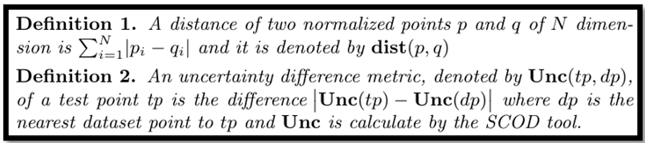
\includegraphics[scale=0.65]{Fig/OOD_def.png}
\caption{Basic definitions.}
\label{fig:Bd}
\end{figure}
With these two definitions, it is feasible to mathematically represent that a test point, $tp$, is similar to a training data if there exists a data point, $dp$, from the training data such that $\bf{dist}(tp, dp) \leq \delta$ and $\bf{dist}(tp, dp) \leq \epsilon$. The imposition of these two inequalities is essential to prevent scenarios where a test point with a low uncertainty metric is erroneously classified as within the distribution, despite being significantly distant from the training dataset. This rationale motivates the following definition, shown in Fig~\ref{fig:OOD}. 
\begin{figure}[ht]
\centering
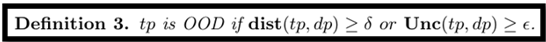
\includegraphics[scale=0.75]{Fig/OOD_def2.png}
\caption{OOD definition.}
\label{fig:OOD}
\end{figure}
These definitions facilitate reframing the task of establishing a threshold value for OOD into the task of determining the generalization performance parameters, $(\delta,\epsilon)$, for managing OOD instances. The computation of these generalization performance parameters is conducted leveraging a DNN model, its associated training dataset, and the SCOD uncertainty metric. 
%This is done next.
 
Second, we calculate $(\delta,\epsilon)$ for data points from the training set and their respective lines between training data points. The computation of the performance parameters occurs through a two-step process, involving the calculation of $\delta$ followed by the computation of $\epsilon$. Initially, $\delta$ is determined as follows: First, for each data point within the training dataset, the closest distance to another data point is computed. Next, $\delta$ is derived as the maximum value among all such closest distances, as illustrated in Fig~\ref{fig:delta}.
\begin{figure}
\centering
\begin{subfigure}{.24\textwidth}
    \centering
    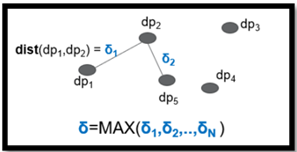
\includegraphics[width=1\linewidth]{Fig/OOD_delta.png}  
    \caption{$\delta$ calculation}
    \label{fig:delta}
\end{subfigure}
\begin{subfigure}{.24\textwidth}
    \centering
    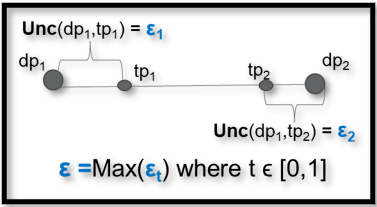
\includegraphics[width=0.93\linewidth]{Fig/OOD_epsilon.png}  
    \caption{$\epsilon$ calculation}
    \label{fig:epsilon}
 \end{subfigure}
\caption{$(\delta,\epsilon)$ calculation}
\label{FIGURE LABEL}
\end{figure}
Next, $\epsilon$ is computed as follows: For each data point within the training dataset, a line is generated connecting it to its closest point. Then, for each generated line, the maximum uncertainty difference metric among its constituent points is calculated using the SCOD tool. This process is depicted in Fig~\ref{fig:epsilon}. Ultimately, $\epsilon$ is determined as the maximum uncertainty metric among all generated lines.   
%Based on the preceding steps, $(\delta,\epsilon)$ could be computed. 
These generalization performance parameters capture the notion that employing the DNN is deemed safe when a test point either is a training data point (trivial case) or lies within a line (reflecting some degree of generalization). However, it is worth noting that the baseline performance parameters may err on the side of caution. %To enhance generalization, the $\delta$ parameter is augmented, a process delineated in the subsequent section.

Third, to further generalize the performance parameters utilizing the $\delta$ parameter, it is necessary to employ a procedure that systematically assesses a set of inputs to identify a subset conducive to generalization. The concept entails leveraging the Operational Design Domain (ODD)~\cite{saej3016,torfah2022learning,irvine2021two} as the overarching set, within which a subset conducive to generalization can be identified. 
The ODD within the DNN framework draws inspiration from autonomous vehicles and robotics. It delineates the specific conditions within which a DNN is engineered and intended to function safely and efficiently. The ODD factors in various considerations, encompassing environmental conditions, temporal aspects, safety constraints, and characteristics of input data. In our pursuit of enhancing the generalization of the performance parameter $\delta$, we will particularly concentrate on the input data characteristics, which entail the distribution and range of features. One methodological approach involves constructing a convex hull within the feature space, represented by the inequality $A.x+b \leq 0$.  The convex hull constitutes the smallest convex set that encompasses all the given points utilized for training. This attribute is pivotal in defining a concise and fundamental set wherein $\delta$ is augmented while maintaining $\epsilon$.  In practical terms, we will verify whether the points within the convex hull exhibit a performance parameter $\epsilon$ equivalent to the points along a line, while possessing a larger $\delta$. 
%Next subsection illustrate this methodology through an illustrative example.


We illustrate this methodology with the analysis of OOD for the Runway Overrun Awareness and Alerting System (ROAAS) specified in ED-250. Here, our primary objective is to obtain the generalization performance parameters. ROAAS is a flight deck alerting system providing crews with situational awareness about the possibility of exceeding the end of the runway during aircraft approach and landing. The ROAAS DNN model comprises ten inputs and three outputs. The objective is to determine the performance parameters 
$(\delta, \epsilon)$ to aid in discerning whether a point is OOD. The computation of these performance parameters unfolds in two steps: the first step involves utilizing a line of the dataset, while the second step entails employing the convex hull of datasets. This phase involves the computation of $\delta$ defined as the maximum of all minimum distances. Fig~\ref{fig:deltaR} posits the value of $\delta$ for ROAAS training data. 
\begin{figure}
%\centering
\begin{subfigure}{.24\textwidth}
    %\centering
    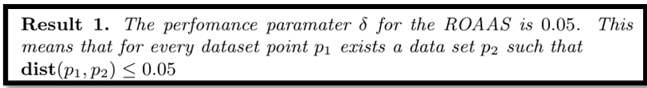
\includegraphics[width=2.0\linewidth]{Fig/OOD_result1.png}  
    \caption{$\delta$ for ROAAS}
    \label{fig:deltaR}
\end{subfigure}
\\
\begin{subfigure}{.24\textwidth}
    %\centering
    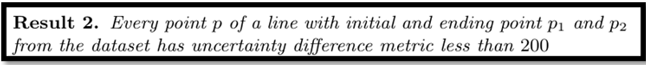
\includegraphics[width=2.0\linewidth]{Fig/OOD_result2.png}  
    \caption{$\epsilon$ for ROAAS}
    \label{fig:epsilonR}
 \end{subfigure}
\caption{$(\delta,\epsilon)$ for ROAAS}
\label{FIGURE LABEL}
\end{figure}
To exemplify this result, consider the data points: $p_1= [8000, 1, 40, 52095, 30, 0,0,0, 161, 0]$ and $p_2= [8000, 1, 40, 52095, 30, 0, 0, 0, 167, 0]$, where the distance between them, denoted by $dist(p_1, p_2)$, equals $0.037$. Subsequently, the calculation of the maximum uncertainty difference metric is executed utilizing the SCOD tool. Fig~\ref{fig:epsilonR} posits the value of $\epsilon$.  To illustrate this result, contemplate the line connecting the data points $dp_1$ and $dp_2$. Each point lying within this line exhibits a performance parameter $\epsilon$ less than $200$, as indicated in Fig~\ref{fig:line}.
\begin{figure}[ht]
\centering
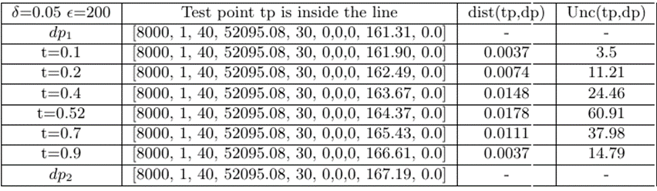
\includegraphics[scale=0.65]{Fig/OOD_result1Exa.png}
\caption{$\epsilon$ for points in a line}
\label{fig:line}
\end{figure}
The baseline values $\delta=0.05$ and $\epsilon=200$ reflect the concept that the model is deemed reliable when the test point either aligns with a training data point (trivial case) or falls within the line (indicating some degree of generalization). A point is classified as OOD if either its $\epsilon$ exceeds $200$ or its $\delta$ surpasses $0.05$. However, this approach may err on the side of caution. To determine the extent to which we can increase $\delta$, we need a benchmark, and the convex hull serves as our reference point. Our goal is to increase $\delta$ based on the convex hull while ensuring $\epsilon \leq 200$. The convex hull is defined by the equation $A.x+b\leq 0$, where $A$ and $b$ were computed using the ROAAS training dataset. Through random testing, we have formulated a value for $\delta$ as shown in Fig~\ref{fig:ConHull}. 
\begin{figure}[ht]
\centering
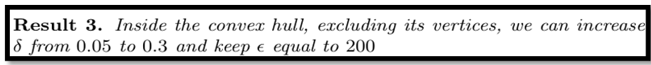
\includegraphics[scale=0.65]{Fig/OOD_result3.png}
\caption{Convex hull}
\label{fig:ConHull}
\end{figure}
Based on this analysis, it is determined that for the ROAAS DNN, a point is considered OOD if either its $\epsilon$ exceeds $200$ or its $\delta$ surpasses $0.3$.



Through the utilization of the SCOD tool for this analysis, the observations suggest that it exhibits a notable degree of adaptability and customization, thereby making it well-suited for a wide spectrum of DNN models. More specifically, it was utilized to compute the $\bf{Unc}$ metric for three Collins models. Its configurability facilitated the uploading of datasets and DNN models, requiring only minor adjustments such as file format conversions. For instance, public Python libraries were leveraged to convert ONNX models to PyTorch. Although employing ROC analysis to calculate the OOD threshold proved impractical for Collins DNN models, an alternative methodology was devised and implemented as outlined in this paper. Thanks to SCOD's flexibility, integrating the SCOD tool with the Python implementation of this methodology was straightforward, enabling the calculation of generalization performance parameters.

\section{Manifold-Based Test Generation}
\label{sec:manifoldBasedTestGeneration}
Neural networks created and deployed in mission critical domains must demonstrate high confidence in their predictions. However, without appropriate training data, it is impossible to evaluate the accuracy of the model. In addition, without considering edge cases and other special scenarios which may or may not be infrequent, the neural networks cannot be trained to handle such cases and make accurate predictions when encountering such scenarios. In high-dimensional input data applications such as image classification, required patterns cannot be easily captured by the available training dataset, which could result in these situations quite easily. 

Manifold-based test generation is a technique that provides a means for capturing the necessary patterns such that the NN can learn these patterns in a low-dimensional manifold space. This is achieved by projecting the data points from a high-dimensional input space to a low-dimensional space. The approach uses a Conditional Variational Autoencoder (CVAE) to capture the manifold space, which is then utilized to generate novel fault-revealing test cases. Note that a unique feature of this approach is that these test cases are generated along with the labels. The resulting fault-revealing test cases can be utilized in two ways: 1) to create a test suite that can evaluate the performance of the neural network, 2) to include the fault revealing test cases as part of the training set such that the neural network performance and accuracy can be improved.

\begin{figure}[h]
%	\vspace{-5mm}
	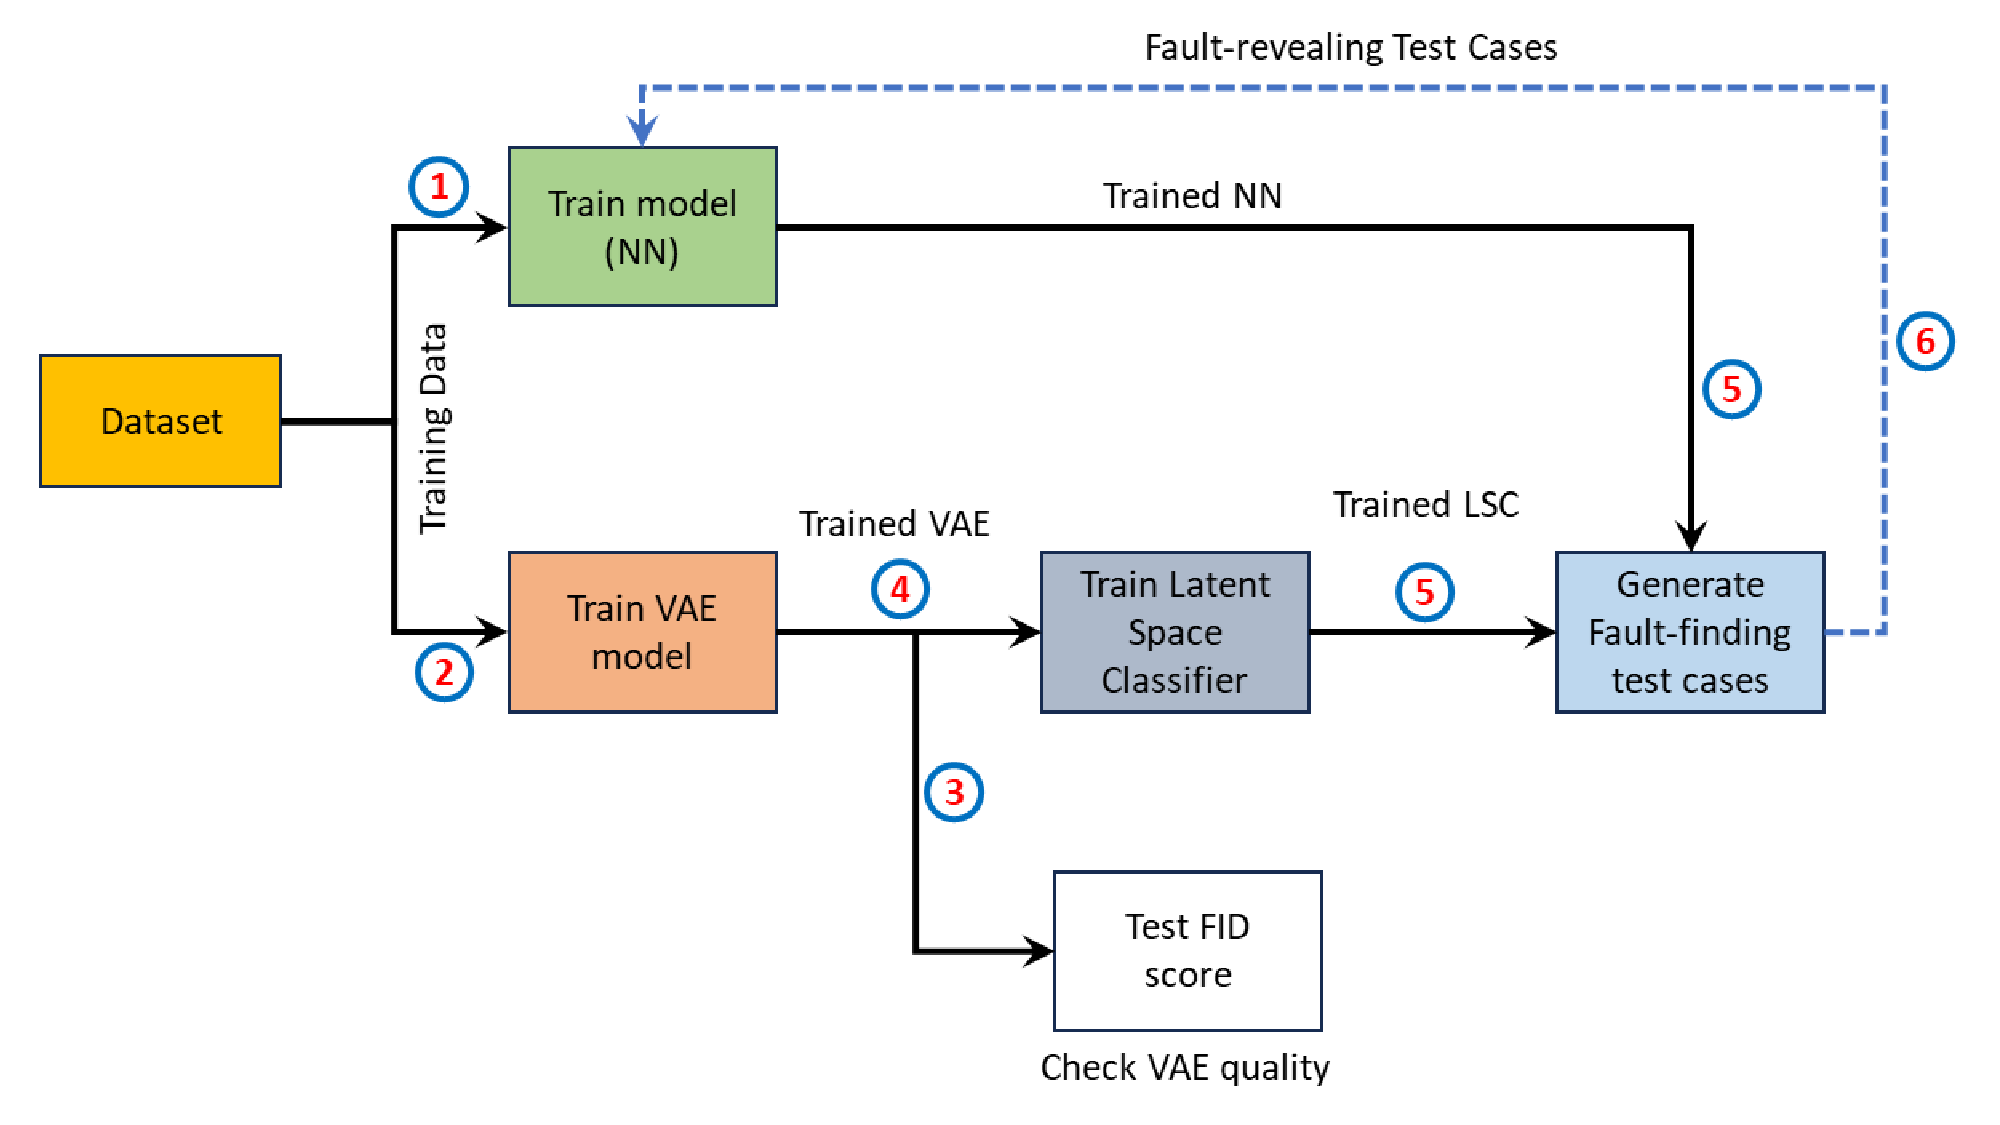
\includegraphics[width=\linewidth]{Fig/manifold_workflow.pdf}
%	\vspace{-20mm}
	\caption{Manifold-based test generation workflow.}
	\label{fig:manifold_workflow}
\end{figure}

Fig~\ref{fig:manifold_workflow} shows the workflow of the manifold based test generation tool. First, the NN is trained using the dataset as shown in Fig~\ref{fig:manifold_workflow} (step 1). The trained NN can be evaluated for its performance using a separate testing dataset, which is not shown in this workflow. Next, a trained VAE is generated by using the same training dataset used for the NN (step 2). Once the trained VAE model is developed, it can then be used to train the Latent Space Classifier (LSC), as shown in Fig~\ref{fig:manifold_workflow} (step 4). Note that if needed, the the quality of the trained VAE can be evaluated by measuring its FID score (step 3). The closer the FID score to zero, the better the trained VAE is assumed to be. Note that this step can also be performed before training the LSC. The LSC is responsible for learning the manifold space. Further, in order to generate fault-revealing test cases from the manifold space, the trained NN and the LSC are passed as an input to the test generation algorithm (step 5). The algorithm then selects the test cases from the manifold space, which includes the label and evaluates it using the NN. If the NN mis-predicts the output, the test case is regarded as a fault-revealing test. The algorithm is able to generate the desired number of faulty test cases, which can be utilized as part of the training data set to re-train the original NN (step 6). Note that in the figure this step is represented using a dashed line because this feature is currently not provided by the tool.

\subsection{Tool evaluation:} We evaluated the tool on the MNIST dataset and followed the workflow as describe in Fig~\ref{fig:manifold_workflow}. Fault revealing test cases can be generated by following various algorithms, but the two utilized in our evaluation are the random test generation and the search-based test generation algorithms. We show the results for both of them below. 

\begin{itemize}
	\item \textit{Random Test Case Generation:} Using this test generation algorithm, the desired number of test cases are generated. However, not all test cases may be fault-revealing. Fig~\ref{fig:random} represents the generation of 50 random test cases. Out of the 50 test cases, only five of these were identified as fault-revealing. The test cases are shown with different color boxes. From Fig~\ref{fig:random}, it is impossible to understand the reasoning behind the selection of the fault-revealing test cases, meaning one cannot tell whether the tool identified the test cases correctly or not. Hence, a visual representation can provide better insight. Therefore, we have generated visual representations for each of the test cases in Fig~\ref{fig:random} as shown in Fig~\ref{fig:random_visual}. %Again, each fault-revealing test case is color-coded for ease of understanding. 
	\begin{figure}[h]
		%	\vspace{-5mm}
		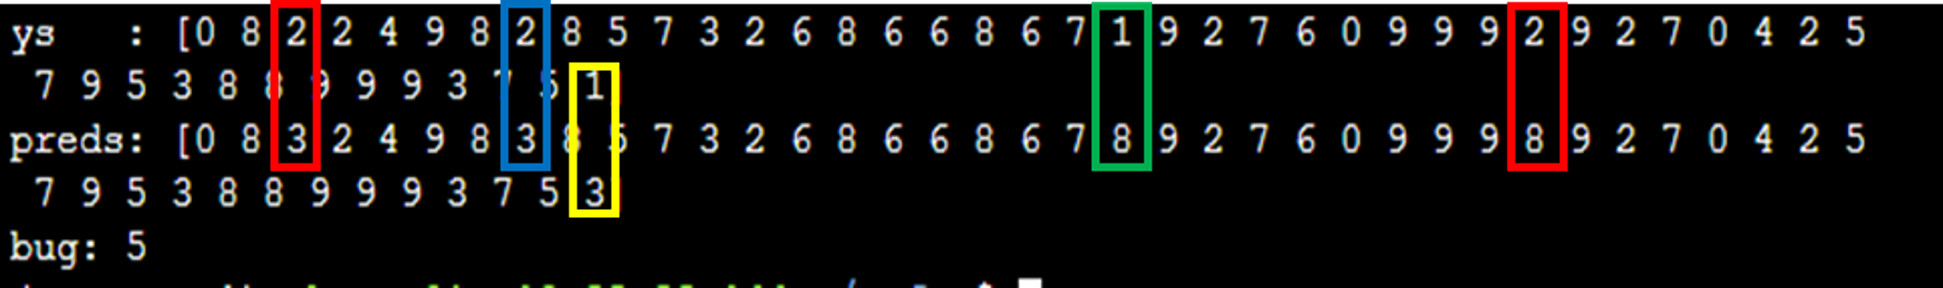
\includegraphics[width=\linewidth]{Fig/random.png}
		%	\vspace{-20mm}
		\caption{Randomly generated test cases.}
		\label{fig:random}
	\end{figure}

	\begin{figure}[h]
		%	\vspace{-5mm}
		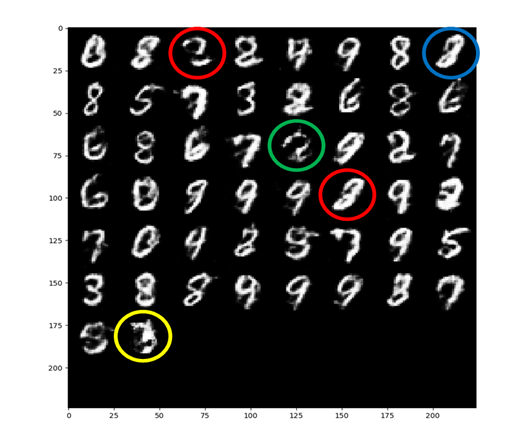
\includegraphics[width=\linewidth]{Fig/random_visual.png}
		%	\vspace{-20mm}
		\caption{Visual representation of randomly generated test cases.}
		\label{fig:random_visual}
	\end{figure}
	\item \textit{Search-Based Test Case Generation:}  Using this test generation algorithm, all the generated test cases are fault-revealing. Fig~\ref{fig:search-based} represents generation of 15 search-based test cases. As shown in the figure, all of the 15 test cases were fault-revealing and they are shown in different color boxes for clarity. Fig~\ref{fig:search_visual} shows the visual representation of each of these fault-revealing test cases. %Again, each of these fault-revealing test cases are color coded for ease of understanding.
	\begin{figure}[h]
		%	\vspace{-5mm}
		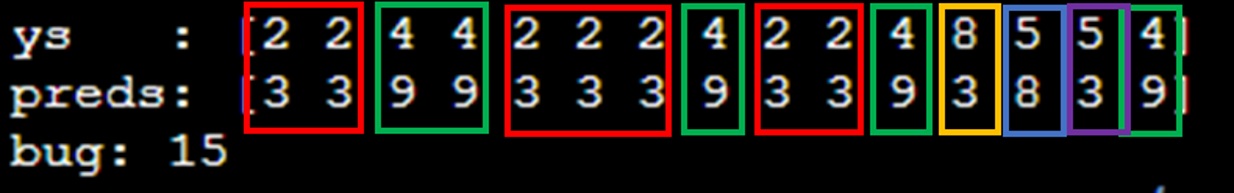
\includegraphics[width=\linewidth]{Fig/search-based.png}
		%	\vspace{-20mm}
		\caption{Search-based generated test cases.}
		\label{fig:search-based}
	\end{figure}

	\begin{figure}[h]
		%	\vspace{-5mm}
		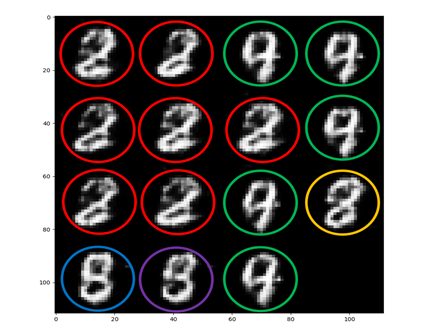
\includegraphics[width=\linewidth]{Fig/search_visual.png}
		%	\vspace{-20mm}
		\caption{Visual representation of search-based generated test cases.}
		\label{fig:search_visual}
	\end{figure}
\end{itemize}
\subsection{Tool Limitations:} Based on our evaluation, the tool provides a unique mechanism for generating fault-revealing test cases for high-dimensional datasets. However, the tool still has the following limitations:
\begin{itemize}
	\item The generated fault-revealing test cases require manual inspection to be considered as part of the training test suite to improve prediction accuracy. As seen from Figures \ref{fig:random_visual} and \ref{fig:search_visual}), it is obvious that some of the predictions and their visual representations do not match and hence require a manual step to analyze the generated test cases. This could become a significant bottleneck when generating a large number of fault-revealing test cases. An automated approach to address this issue would make the tool significantly more useful. 
	\item The tool was developed as a prototype to demonstrate the proof of concept and still requires several updates to completely become usable in this space. For instance, the algorithm for search-based test generation was modified slightly to capture only fault-revealing test cases. 
	\item The tool is currently capable of working with MNIST, CIFAR, FASHION, and EMNIST datasets. To use other datasets as inputs, minor tool modifications are required.
	\item The approach works on high-dimensional datasets; however, for low-dimensional classification problems the tool is unable to handle the datasets appropriately. We believe the approach is sound and should be easily applicable to low-dimensional classification problems. This could easily enable even the neural networks in other classification problem domains to acquire better accuracy. However, the tool is currently unable to handle low-dimensional training datasets and therefore requires modification. The extent of needed modifications was not evaluated as part of our process.
\end{itemize}


\section{Property Inference}
\label{sec:propertyInference}
The Prophecy tool developed by NASA\cite{Gopinath2019FindingII,8952519} derives invariant properties of feed-forward neural networks, showcasing the networks' capacity to learn decision logic from neuron activation patterns. The method involves identifying decision patterns as network invariants connected to specific outputs, achieved through extracting input invariants and layer invariants. Formal verification utilizing decision procedures like Reluplex~\cite{10.1007/s10703-021-00363-7}, a predecessor of Marabou, ensures that given invariants lead to desired outcomes, enhancing explainability, robustness, and aiding in network simplification and distillation. However, scalability issues, particularly with formal verification, pose significant challenges, such as timeouts when dealing with large-scale networks. 

In evaluating the Prophecy formal verification approach, we applied it to the Flight Trajectory Optimization (FTO) application.  FTO can be used to help aircraft navigate around hazardous weather conditions. 
Challenges like scalability, lack of modularity, and outdated documentation hindered progress. An updated version of Prophecy~\cite{safednn-nasa} integrated Marabou for the formal verification step, and a parallel execution algorithm to enhance scalability, addressing some of the challenges encountered. Initial tests on ACAS-Xu~\cite{10.1007/978-3-030-62822-2_4} showed promising results, with Marabou successfully verifying some properties in a significantly reduced timeframe compared to applying Reluplex directly. 

For example, Reluplex may need 12 hours while trying to verify the Clear of Conflict (CoC) property over certain domain invariants of large size. However, the tool successfully verified the same ACAS-Xu CoC properties in approximately 3.5 hours using Marabou over similar invariants.

The most resource-intensive step in the formal verification process involved refining initial convex hull guesses, aiming to eliminate adversarial examples and ensure robust invariants. 

We found that optimizing Prophecy's performance is crucial before deploying the algorithm for applications where the complexity of the formal verification step increases substantially compared to ACAS-Xu.

Techniques like using $\alpha$-$\beta$-CROWN could enhance the refinement step, albeit with limitations. %For instance, unlike Marabou, $\alpha$-$\beta$-CROWN may not handle linear input constraints.
Additionally, more efforts are needed to resolve issues with corrupted invariants.


Future directions involve exploring transformer architecture, such as GPT embedding models\cite{GPT4} and classifiers, to improve the quality of the initial convex hull approximations and reduce the need for redundant formal checks. If successful, this approach could offer scalable solutions for larger datasets and dimensions, enhancing the generalizability of formal verification methods in NN analysis.

\section{Conclusion}
\label{sec:conclusion}
Collins researchers and product engineers are exploring many applications of machine learning.  In some cases, the goal is to implement new aircraft functionality using the unique capabilities of ML.  In other cases, the goal is to use a neural network to create a more time- or memory-efficient implementation of an existing function.  

A variety of assurance technologies have been developed and investigated on the DARPA Assured Autonomy program and related efforts.  These include new approaches for testing and completeness metrics, formal analysis of neural networks, input domain shift assessment, and run-time monitoring and enforcement architectures.
For each selected ML application, we determined one or more AA technologies that can be used to satisfy the relevant certification objectives.  We evaluated the effectiveness of the technologies and the evidence produced.

% What is our overall impression of these tools?
In general, we believe all the approaches covered in this paper can play a role in assuring low-complexity, low-DAL products.  The manifold-based test generation and property inference tools have not yet reached the necessary maturity levels to be used on programs of record, but their underlying methodologies show promise.  
We plan to share these findings with certification authorities to obtain feedback.



\bibliographystyle{IEEEtran}
%\bibliography{biblio}
\bibliography{biblioOOD}


\end{document}
